% Options for packages loaded elsewhere
\PassOptionsToPackage{unicode}{hyperref}
\PassOptionsToPackage{hyphens}{url}
%
\documentclass[
  11pt,
  ignorenonframetext,
]{beamer}
\usepackage{pgfpages}
\setbeamertemplate{caption}[numbered]
\setbeamertemplate{caption label separator}{: }
\setbeamercolor{caption name}{fg=normal text.fg}
\beamertemplatenavigationsymbolsempty
% Prevent slide breaks in the middle of a paragraph
\widowpenalties 1 10000
\raggedbottom
\setbeamertemplate{part page}{
  \centering
  \begin{beamercolorbox}[sep=16pt,center]{part title}
    \usebeamerfont{part title}\insertpart\par
  \end{beamercolorbox}
}
\setbeamertemplate{section page}{
  \centering
  \begin{beamercolorbox}[sep=12pt,center]{part title}
    \usebeamerfont{section title}\insertsection\par
  \end{beamercolorbox}
}
\setbeamertemplate{subsection page}{
  \centering
  \begin{beamercolorbox}[sep=8pt,center]{part title}
    \usebeamerfont{subsection title}\insertsubsection\par
  \end{beamercolorbox}
}
\AtBeginPart{
  \frame{\partpage}
}
\AtBeginSection{
  \ifbibliography
  \else
    \frame{\sectionpage}
  \fi
}
\AtBeginSubsection{
  \frame{\subsectionpage}
}
\usepackage{amsmath,amssymb}
\usepackage{iftex}
\ifPDFTeX
  \usepackage[T1]{fontenc}
  \usepackage[utf8]{inputenc}
  \usepackage{textcomp} % provide euro and other symbols
\else % if luatex or xetex
  \usepackage{unicode-math} % this also loads fontspec
  \defaultfontfeatures{Scale=MatchLowercase}
  \defaultfontfeatures[\rmfamily]{Ligatures=TeX,Scale=1}
\fi
\usepackage{lmodern}
\usetheme[]{metropolis}
\ifPDFTeX\else
  % xetex/luatex font selection
\fi
% Use upquote if available, for straight quotes in verbatim environments
\IfFileExists{upquote.sty}{\usepackage{upquote}}{}
\IfFileExists{microtype.sty}{% use microtype if available
  \usepackage[]{microtype}
  \UseMicrotypeSet[protrusion]{basicmath} % disable protrusion for tt fonts
}{}
\makeatletter
\@ifundefined{KOMAClassName}{% if non-KOMA class
  \IfFileExists{parskip.sty}{%
    \usepackage{parskip}
  }{% else
    \setlength{\parindent}{0pt}
    \setlength{\parskip}{6pt plus 2pt minus 1pt}}
}{% if KOMA class
  \KOMAoptions{parskip=half}}
\makeatother
\usepackage{xcolor}
\newif\ifbibliography
\usepackage{color}
\usepackage{fancyvrb}
\newcommand{\VerbBar}{|}
\newcommand{\VERB}{\Verb[commandchars=\\\{\}]}
\DefineVerbatimEnvironment{Highlighting}{Verbatim}{commandchars=\\\{\}}
% Add ',fontsize=\small' for more characters per line
\newenvironment{Shaded}{}{}
\newcommand{\AlertTok}[1]{\textcolor[rgb]{1.00,0.00,0.00}{\textbf{#1}}}
\newcommand{\AnnotationTok}[1]{\textcolor[rgb]{0.38,0.63,0.69}{\textbf{\textit{#1}}}}
\newcommand{\AttributeTok}[1]{\textcolor[rgb]{0.49,0.56,0.16}{#1}}
\newcommand{\BaseNTok}[1]{\textcolor[rgb]{0.25,0.63,0.44}{#1}}
\newcommand{\BuiltInTok}[1]{\textcolor[rgb]{0.00,0.50,0.00}{#1}}
\newcommand{\CharTok}[1]{\textcolor[rgb]{0.25,0.44,0.63}{#1}}
\newcommand{\CommentTok}[1]{\textcolor[rgb]{0.38,0.63,0.69}{\textit{#1}}}
\newcommand{\CommentVarTok}[1]{\textcolor[rgb]{0.38,0.63,0.69}{\textbf{\textit{#1}}}}
\newcommand{\ConstantTok}[1]{\textcolor[rgb]{0.53,0.00,0.00}{#1}}
\newcommand{\ControlFlowTok}[1]{\textcolor[rgb]{0.00,0.44,0.13}{\textbf{#1}}}
\newcommand{\DataTypeTok}[1]{\textcolor[rgb]{0.56,0.13,0.00}{#1}}
\newcommand{\DecValTok}[1]{\textcolor[rgb]{0.25,0.63,0.44}{#1}}
\newcommand{\DocumentationTok}[1]{\textcolor[rgb]{0.73,0.13,0.13}{\textit{#1}}}
\newcommand{\ErrorTok}[1]{\textcolor[rgb]{1.00,0.00,0.00}{\textbf{#1}}}
\newcommand{\ExtensionTok}[1]{#1}
\newcommand{\FloatTok}[1]{\textcolor[rgb]{0.25,0.63,0.44}{#1}}
\newcommand{\FunctionTok}[1]{\textcolor[rgb]{0.02,0.16,0.49}{#1}}
\newcommand{\ImportTok}[1]{\textcolor[rgb]{0.00,0.50,0.00}{\textbf{#1}}}
\newcommand{\InformationTok}[1]{\textcolor[rgb]{0.38,0.63,0.69}{\textbf{\textit{#1}}}}
\newcommand{\KeywordTok}[1]{\textcolor[rgb]{0.00,0.44,0.13}{\textbf{#1}}}
\newcommand{\NormalTok}[1]{#1}
\newcommand{\OperatorTok}[1]{\textcolor[rgb]{0.40,0.40,0.40}{#1}}
\newcommand{\OtherTok}[1]{\textcolor[rgb]{0.00,0.44,0.13}{#1}}
\newcommand{\PreprocessorTok}[1]{\textcolor[rgb]{0.74,0.48,0.00}{#1}}
\newcommand{\RegionMarkerTok}[1]{#1}
\newcommand{\SpecialCharTok}[1]{\textcolor[rgb]{0.25,0.44,0.63}{#1}}
\newcommand{\SpecialStringTok}[1]{\textcolor[rgb]{0.73,0.40,0.53}{#1}}
\newcommand{\StringTok}[1]{\textcolor[rgb]{0.25,0.44,0.63}{#1}}
\newcommand{\VariableTok}[1]{\textcolor[rgb]{0.10,0.09,0.49}{#1}}
\newcommand{\VerbatimStringTok}[1]{\textcolor[rgb]{0.25,0.44,0.63}{#1}}
\newcommand{\WarningTok}[1]{\textcolor[rgb]{0.38,0.63,0.69}{\textbf{\textit{#1}}}}
\usepackage{graphicx}
\makeatletter
\def\maxwidth{\ifdim\Gin@nat@width>\linewidth\linewidth\else\Gin@nat@width\fi}
\def\maxheight{\ifdim\Gin@nat@height>\textheight\textheight\else\Gin@nat@height\fi}
\makeatother
% Scale images if necessary, so that they will not overflow the page
% margins by default, and it is still possible to overwrite the defaults
% using explicit options in \includegraphics[width, height, ...]{}
\setkeys{Gin}{width=\maxwidth,height=\maxheight,keepaspectratio}
% Set default figure placement to htbp
\makeatletter
\def\fps@figure{htbp}
\makeatother
\setlength{\emergencystretch}{3em} % prevent overfull lines
\providecommand{\tightlist}{%
  \setlength{\itemsep}{0pt}\setlength{\parskip}{0pt}}
\setcounter{secnumdepth}{-\maxdimen} % remove section numbering
\ifLuaTeX
  \usepackage{selnolig}  % disable illegal ligatures
\fi
\IfFileExists{bookmark.sty}{\usepackage{bookmark}}{\usepackage{hyperref}}
\IfFileExists{xurl.sty}{\usepackage{xurl}}{} % add URL line breaks if available
\urlstyle{same}
\hypersetup{
  pdftitle={Metapoblaciones},
  pdfauthor={Gerardo Martín},
  hidelinks,
  pdfcreator={LaTeX via pandoc}}

\title{Metapoblaciones}
\subtitle{Integración con \texttt{deSolve}}
\author{Gerardo Martín}
\date{28-07-2023}

\begin{document}
\frame{\titlepage}

\hypertarget{integraciuxf3n-con-paquete-desolve}{%
\section{\texorpdfstring{Integración con paquete
\texttt{deSolve}}{Integración con paquete deSolve}}\label{integraciuxf3n-con-paquete-desolve}}

\hypertarget{necesidad-real}{%
\subsection{Necesidad real}\label{necesidad-real}}

\begin{frame}{Necesidad real}
\begin{figure}
\centering
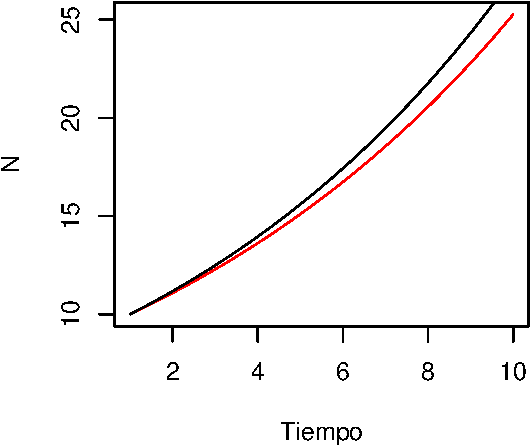
\includegraphics{deSolve_files/figure-beamer/unnamed-chunk-1-1.pdf}
\caption{Línea negra es la solución analítica. Roja es solución de
Euler}
\end{figure}
\end{frame}

\hypertarget{necesidad-real-1}{%
\subsection{Necesidad real}\label{necesidad-real-1}}

\begin{frame}[fragile]{Necesidad real}
\begin{itemize}
\item
  El método de Euler es muy inexacto
\item
  El error de integración se acumula
\item
  Se puede controlar, disminuyendo \(h\), pero se vuelve leeento
\item
  Métodos como Runge-Kutta de 2 y 4 pasos tienen menos error

  \begin{itemize}
  \tightlist
  \item
    Adams-Bashford son más sofisticados y rápidos
  \end{itemize}
\item
  Están implementados en paquete \texttt{deSolve} de \textbf{R}
\end{itemize}
\end{frame}

\hypertarget{uso-de-desolve}{%
\subsection{\texorpdfstring{Uso de
\texttt{deSolve}}{Uso de deSolve}}\label{uso-de-desolve}}

\begin{frame}[fragile]{Uso de \texttt{deSolve}}
\begin{enumerate}
\item
  Crear función del modelo
\item
  Crear objeto con valores de parámetros
\item
  Establecer condiciones iniciales
\item
  Correr simulación confunción \texttt{lsoda}
\end{enumerate}
\end{frame}

\hypertarget{la-funciuxf3n-del-modelo}{%
\section{La función del modelo}\label{la-funciuxf3n-del-modelo}}

\hypertarget{crear-funciones-con-r}{%
\subsection{\texorpdfstring{Crear funciones con
\textbf{R}}{Crear funciones con R}}\label{crear-funciones-con-r}}

\begin{frame}[fragile]{Crear funciones con \textbf{R}}
\begin{itemize}
\item
  Funciones: código que contiene órdenes para R
\item
  Se suelen crear cuando se necesita repetir una operación
\item
  Sintaxis:
\end{itemize}

\begin{Shaded}
\begin{Highlighting}[]
\NormalTok{f }\OtherTok{\textless{}{-}} \ControlFlowTok{function}\NormalTok{(x)\{}\FunctionTok{print}\NormalTok{(x)\}}
\end{Highlighting}
\end{Shaded}

\begin{itemize}
\item
  Para especificar una función se crea un objeto que contentrá la
  órdenes
\item
  El objeto se llama, y entre \texttt{()} se especifican los argumentos
\end{itemize}
\end{frame}

\hypertarget{crear-funciones-con-r-1}{%
\subsection{\texorpdfstring{Crear funciones con
\textbf{R}}{Crear funciones con R}}\label{crear-funciones-con-r-1}}

\begin{frame}[fragile]{Crear funciones con \textbf{R}}
\begin{itemize}
\item
  La función \texttt{f} requiere un sólo argumento de nombre \texttt{x}
\item
  Una vez que llamamos \texttt{a} tenemos que especificar el valor de
  \texttt{x}, y \textbf{R} imprimirá el resultado:
\end{itemize}

\begin{Shaded}
\begin{Highlighting}[]
\FunctionTok{f}\NormalTok{(}\DecValTok{1}\NormalTok{)}
\end{Highlighting}
\end{Shaded}

\begin{verbatim}
## [1] 1
\end{verbatim}
\end{frame}

\hypertarget{funciones-con-muxe1s-argumentos}{%
\subsection{Funciones con más
argumentos}\label{funciones-con-muxe1s-argumentos}}

\begin{frame}[fragile]{Funciones con más argumentos}
Las funciones pueden tomar más de un argumento:

\begin{Shaded}
\begin{Highlighting}[]
\NormalTok{g }\OtherTok{\textless{}{-}} \ControlFlowTok{function}\NormalTok{(x, y)\{}\FunctionTok{print}\NormalTok{(x }\SpecialCharTok{+}\NormalTok{ y)\}}
\FunctionTok{g}\NormalTok{(}\DecValTok{1}\NormalTok{, }\DecValTok{3}\NormalTok{)}
\end{Highlighting}
\end{Shaded}

\begin{verbatim}
## [1] 4
\end{verbatim}

Ó utilizar argumentos de más de un tipo (números y caracteres)

\begin{Shaded}
\begin{Highlighting}[]
\NormalTok{h }\OtherTok{\textless{}{-}} \ControlFlowTok{function}\NormalTok{(x, y, }\AttributeTok{z =} \StringTok{"a"}\NormalTok{)\{}\FunctionTok{print}\NormalTok{(}\FunctionTok{paste0}\NormalTok{(x }\SpecialCharTok{+}\NormalTok{ y, }\StringTok{"="}\NormalTok{, z))\}}
\FunctionTok{h}\NormalTok{(}\DecValTok{1}\NormalTok{, }\DecValTok{2}\NormalTok{, }\StringTok{"b"}\NormalTok{)}
\end{Highlighting}
\end{Shaded}

\begin{verbatim}
## [1] "3=b"
\end{verbatim}
\end{frame}

\hypertarget{especificando-la-funciuxf3n-del-modelo-exponencial}{%
\subsection{Especificando la función del modelo
exponencial}\label{especificando-la-funciuxf3n-del-modelo-exponencial}}

\begin{frame}[fragile]{Especificando la función del modelo exponencial}
La función necesita tres argumentos, el tiempo \texttt{t}, los valores
\texttt{y} y los parámetros del modelo:

\begin{Shaded}
\begin{Highlighting}[]
\NormalTok{expon }\OtherTok{\textless{}{-}} \ControlFlowTok{function}\NormalTok{(t, y, parms)\{}
  
\NormalTok{\}}
\end{Highlighting}
\end{Shaded}

Entre los corchetes \texttt{\{\}}, especificamos las posiciones de
\texttt{y} que contienen las variables de estado (\texttt{N})

\begin{Shaded}
\begin{Highlighting}[]
\NormalTok{N }\OtherTok{\textless{}{-}}\NormalTok{ y[}\DecValTok{1}\NormalTok{]}
\end{Highlighting}
\end{Shaded}

las operaciones de que consiste el modelo, el exponencial:

\begin{Shaded}
\begin{Highlighting}[]
\NormalTok{dN }\OtherTok{\textless{}{-}}\NormalTok{ r }\SpecialCharTok{*}\NormalTok{ N}
\end{Highlighting}
\end{Shaded}
\end{frame}

\hypertarget{funciuxf3n-completa-del-modelo}{%
\subsection{Función completa del
modelo}\label{funciuxf3n-completa-del-modelo}}

\begin{frame}[fragile]{Función completa del modelo}
\begin{Shaded}
\begin{Highlighting}[]
\NormalTok{expon }\OtherTok{\textless{}{-}} \ControlFlowTok{function}\NormalTok{(t, y, parms)\{}
\NormalTok{  N }\OtherTok{\textless{}{-}}\NormalTok{ y[}\DecValTok{1}\NormalTok{]}
  \FunctionTok{with}\NormalTok{(parametros,\{}
\NormalTok{    dN }\OtherTok{\textless{}{-}}\NormalTok{ r }\SpecialCharTok{*}\NormalTok{ N}
    \FunctionTok{return}\NormalTok{(}\FunctionTok{list}\NormalTok{(dN))}
\NormalTok{  \})}
\NormalTok{\}}
\end{Highlighting}
\end{Shaded}

los argumentos \texttt{t} y \texttt{parms} los veremos a continuación
\end{frame}

\hypertarget{argumentos-de-la-funciuxf3n}{%
\subsection{Argumentos de la
función}\label{argumentos-de-la-funciuxf3n}}

\begin{frame}[fragile]{Argumentos de la función}
\texttt{t} es una secuencia de valores del tiempo:

\begin{Shaded}
\begin{Highlighting}[]
\NormalTok{t }\OtherTok{\textless{}{-}} \FunctionTok{seq}\NormalTok{(}\DecValTok{0}\NormalTok{, }\DecValTok{10}\NormalTok{, }\AttributeTok{by =} \FloatTok{0.1}\NormalTok{)}
\end{Highlighting}
\end{Shaded}

\texttt{y} es un objeto que sólo contiene las condiciones iniciales:

\begin{Shaded}
\begin{Highlighting}[]
\NormalTok{y }\OtherTok{\textless{}{-}} \DecValTok{10}
\end{Highlighting}
\end{Shaded}

\texttt{parms} es una lista que contiene los valores que cada parámetro:

\begin{Shaded}
\begin{Highlighting}[]
\NormalTok{parametros }\OtherTok{\textless{}{-}} \FunctionTok{list}\NormalTok{(}\AttributeTok{r =} \FloatTok{0.1}\NormalTok{)}
\end{Highlighting}
\end{Shaded}
\end{frame}

\hypertarget{llamando-desolve-para-correr-simulaciuxf3n}{%
\subsection{\texorpdfstring{Llamando \texttt{deSolve} para correr
simulación}{Llamando deSolve para correr simulación}}\label{llamando-desolve-para-correr-simulaciuxf3n}}

\begin{frame}[fragile]{Llamando \texttt{deSolve} para correr simulación}
\begin{Shaded}
\begin{Highlighting}[]
\FunctionTok{library}\NormalTok{(deSolve)}

\NormalTok{sim }\OtherTok{\textless{}{-}} \FunctionTok{lsoda}\NormalTok{(}\AttributeTok{y =}\NormalTok{ y, }\AttributeTok{times =}\NormalTok{ t, }\AttributeTok{parms =}\NormalTok{ parametros, }\AttributeTok{func =}\NormalTok{ expon)}
\end{Highlighting}
\end{Shaded}

\texttt{lsoda} es la función de \texttt{deSolve} que hará la simulación

Los argumentos, ¿se explican solos?
\end{frame}

\hypertarget{explorando-la-salida-de-lsoda}{%
\subsection{\texorpdfstring{Explorando la salida de
\texttt{lsoda}}{Explorando la salida de lsoda}}\label{explorando-la-salida-de-lsoda}}

\begin{frame}[fragile]{Explorando la salida de \texttt{lsoda}}
Podemos imprimir las primeras filas

\begin{Shaded}
\begin{Highlighting}[]
\FunctionTok{head}\NormalTok{(sim)}
\end{Highlighting}
\end{Shaded}

\begin{verbatim}
##      time        1
## [1,]  0.0 10.00000
## [2,]  0.1 10.10050
## [3,]  0.2 10.20202
## [4,]  0.3 10.30455
## [5,]  0.4 10.40811
## [6,]  0.5 10.51271
\end{verbatim}
\end{frame}

\hypertarget{explorando-la-salida-de-lsoda-1}{%
\subsection{\texorpdfstring{Explorando la salida de
\texttt{lsoda}}{Explorando la salida de lsoda}}\label{explorando-la-salida-de-lsoda-1}}

\begin{frame}{Explorando la salida de \texttt{lsoda}}
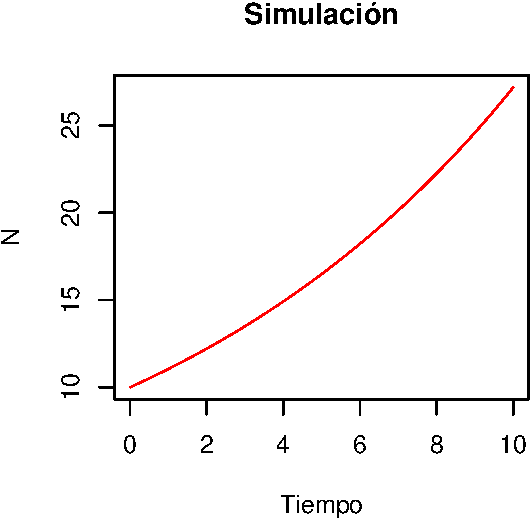
\includegraphics{deSolve_files/figure-beamer/unnamed-chunk-15-1.pdf}
\end{frame}

\hypertarget{simulaciuxf3n-de-un-modelo-con-muxe1s-de-un-paruxe1metro}{%
\section{Simulación de un modelo con más de un
parámetro}\label{simulaciuxf3n-de-un-modelo-con-muxe1s-de-un-paruxe1metro}}

\hypertarget{funciuxf3n-del-modelo-de-levins}{%
\subsection{Función del modelo de
levins}\label{funciuxf3n-del-modelo-de-levins}}

\begin{frame}[fragile]{Función del modelo de levins}
\begin{Shaded}
\begin{Highlighting}[]
\NormalTok{levins }\OtherTok{\textless{}{-}} \ControlFlowTok{function}\NormalTok{(t, y, parms)\{}
\NormalTok{  p }\OtherTok{\textless{}{-}}\NormalTok{ y[}\DecValTok{1}\NormalTok{]}
  \FunctionTok{with}\NormalTok{(parms, \{}
\NormalTok{    dp }\OtherTok{\textless{}{-}}\NormalTok{ c}\SpecialCharTok{*}\NormalTok{p}\SpecialCharTok{*}\NormalTok{(}\DecValTok{1}\SpecialCharTok{{-}}\NormalTok{p) }\SpecialCharTok{{-}}\NormalTok{ e}\SpecialCharTok{*}\NormalTok{p}
    \FunctionTok{return}\NormalTok{(}\FunctionTok{list}\NormalTok{(dp))}
\NormalTok{  \})}
\NormalTok{\}}
\end{Highlighting}
\end{Shaded}
\end{frame}

\hypertarget{t-y-parms}{%
\subsection{\texorpdfstring{\texttt{t}, \texttt{y},
\texttt{parms}}{t, y, parms}}\label{t-y-parms}}

\begin{frame}[fragile]{\texttt{t}, \texttt{y}, \texttt{parms}}
\begin{Shaded}
\begin{Highlighting}[]
\NormalTok{t }\OtherTok{\textless{}{-}} \FunctionTok{seq}\NormalTok{(}\DecValTok{0}\NormalTok{, }\DecValTok{100}\NormalTok{, }\AttributeTok{by =} \FloatTok{0.1}\NormalTok{)}
\NormalTok{y }\OtherTok{\textless{}{-}} \FloatTok{0.1}
\NormalTok{parms }\OtherTok{\textless{}{-}} \FunctionTok{list}\NormalTok{(}\AttributeTok{c =} \FloatTok{0.5}\NormalTok{, }\AttributeTok{e =} \FloatTok{0.05}\NormalTok{)}
\end{Highlighting}
\end{Shaded}
\end{frame}

\hypertarget{simulando-levins}{%
\subsection{Simulando Levins}\label{simulando-levins}}

\begin{frame}[fragile]{Simulando Levins}
\begin{Shaded}
\begin{Highlighting}[]
\NormalTok{sim.lev }\OtherTok{\textless{}{-}} \FunctionTok{lsoda}\NormalTok{(}\AttributeTok{y =}\NormalTok{ y, }\AttributeTok{times =}\NormalTok{ t, }
                 \AttributeTok{parms =}\NormalTok{ parms,}
                 \AttributeTok{func =}\NormalTok{ levins)}
\FunctionTok{head}\NormalTok{(sim.lev)}
\end{Highlighting}
\end{Shaded}

\begin{verbatim}
##      time         1
## [1,]  0.0 0.1000000
## [2,]  0.1 0.1040708
## [3,]  0.2 0.1082849
## [4,]  0.3 0.1126455
## [5,]  0.4 0.1171553
## [6,]  0.5 0.1218178
\end{verbatim}
\end{frame}

\hypertarget{gruxe1fica-de-las-simulaciones}{%
\subsection{Gráfica de las
simulaciones}\label{gruxe1fica-de-las-simulaciones}}

\begin{frame}{Gráfica de las simulaciones}
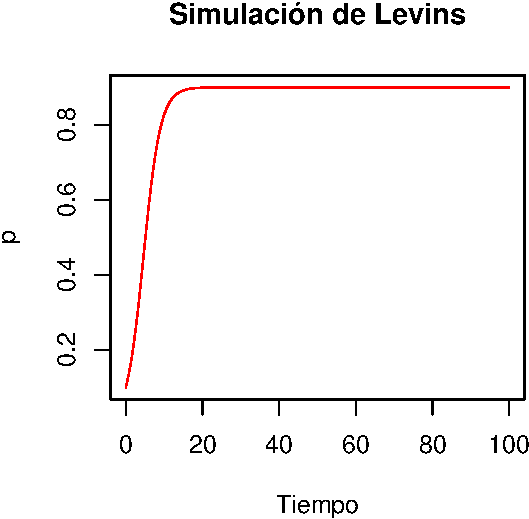
\includegraphics{deSolve_files/figure-beamer/unnamed-chunk-19-1.pdf}
\end{frame}

\hypertarget{simulaciuxf3n-de-un-modelo-con-dos-variables-de-estado}{%
\section{Simulación de un modelo con dos variables de
estado}\label{simulaciuxf3n-de-un-modelo-con-dos-variables-de-estado}}

\hypertarget{el-modelo}{%
\subsection{El modelo}\label{el-modelo}}

\begin{frame}{El modelo}
\begin{align}
    \frac{N_1}{dt} &= r N_1 (1-N_1/K) + i N_2-e N_1 \\
    \frac{N_2}{dt} &= r N_2 (1-N_2/K) + i N_1-e N_2
\end{align}
\end{frame}

\hypertarget{la-funciuxf3n}{%
\subsection{La función}\label{la-funciuxf3n}}

\begin{frame}[fragile]{La función}
\begin{Shaded}
\begin{Highlighting}[]
\NormalTok{mig }\OtherTok{\textless{}{-}} \ControlFlowTok{function}\NormalTok{(t, y, parms)\{}
  \FunctionTok{with}\NormalTok{(parms, \{}
\NormalTok{      N1 }\OtherTok{\textless{}{-}}\NormalTok{ y[}\DecValTok{1}\NormalTok{]}
\NormalTok{      N2 }\OtherTok{\textless{}{-}}\NormalTok{ y[}\DecValTok{2}\NormalTok{]}
  
\NormalTok{    dN1 }\OtherTok{\textless{}{-}}\NormalTok{ r }\SpecialCharTok{*}\NormalTok{ N1 }\SpecialCharTok{*}\NormalTok{ (}\DecValTok{1} \SpecialCharTok{{-}}\NormalTok{ N1}\SpecialCharTok{/}\NormalTok{K) }\SpecialCharTok{+}\NormalTok{ m2 }\SpecialCharTok{*}\NormalTok{ N2 }\SpecialCharTok{{-}}\NormalTok{ m1 }\SpecialCharTok{*}\NormalTok{ N1}
\NormalTok{    dN2 }\OtherTok{\textless{}{-}}\NormalTok{ r }\SpecialCharTok{*}\NormalTok{ N2 }\SpecialCharTok{*}\NormalTok{ (}\DecValTok{1} \SpecialCharTok{{-}}\NormalTok{ N2}\SpecialCharTok{/}\NormalTok{K) }\SpecialCharTok{+}\NormalTok{ m1 }\SpecialCharTok{*}\NormalTok{ N1 }\SpecialCharTok{{-}}\NormalTok{ m2 }\SpecialCharTok{*}\NormalTok{ N2}
    
    \FunctionTok{return}\NormalTok{(}\FunctionTok{list}\NormalTok{(}\FunctionTok{c}\NormalTok{(dN1, dN2)))}
\NormalTok{  \})}
\NormalTok{\}}
\end{Highlighting}
\end{Shaded}
\end{frame}

\hypertarget{t-y-parms-1}{%
\subsection{\texorpdfstring{\texttt{t}, \texttt{y},
\texttt{parms}}{t, y, parms}}\label{t-y-parms-1}}

\begin{frame}[fragile]{\texttt{t}, \texttt{y}, \texttt{parms}}
\begin{Shaded}
\begin{Highlighting}[]
\NormalTok{t }\OtherTok{\textless{}{-}} \FunctionTok{seq}\NormalTok{(}\DecValTok{0}\NormalTok{, }\DecValTok{10}\NormalTok{, }\AttributeTok{by =} \FloatTok{0.1}\NormalTok{)}
\NormalTok{y }\OtherTok{\textless{}{-}} \FunctionTok{c}\NormalTok{(}\AttributeTok{N1 =} \DecValTok{10}\NormalTok{, }\AttributeTok{N2 =} \DecValTok{0}\NormalTok{)}
\NormalTok{parms }\OtherTok{\textless{}{-}} \FunctionTok{list}\NormalTok{(}\AttributeTok{r =} \FloatTok{0.5}\NormalTok{, }\AttributeTok{K =} \DecValTok{25}\NormalTok{,}
              \AttributeTok{m1 =} \FloatTok{0.1}\NormalTok{, }\AttributeTok{m2 =} \FloatTok{0.2}\NormalTok{)}
\end{Highlighting}
\end{Shaded}
\end{frame}

\hypertarget{la-simulaciuxf3n}{%
\subsection{La simulación}\label{la-simulaciuxf3n}}

\begin{frame}[fragile]{La simulación}
\begin{Shaded}
\begin{Highlighting}[]
\NormalTok{sim.mig }\OtherTok{\textless{}{-}} \FunctionTok{lsoda}\NormalTok{(}\AttributeTok{y =}\NormalTok{ y, }\AttributeTok{times =}\NormalTok{ t, }
                 \AttributeTok{parms =}\NormalTok{ parms,}
                 \AttributeTok{func =}\NormalTok{ mig)}
\FunctionTok{head}\NormalTok{(sim.mig, }\DecValTok{3}\NormalTok{)}
\end{Highlighting}
\end{Shaded}

\begin{verbatim}
##      time       N1        N2
## [1,]  0.0 10.00000 0.0000000
## [2,]  0.1 10.20099 0.1025226
## [3,]  0.2 10.40392 0.2101706
\end{verbatim}
\end{frame}

\hypertarget{preparando-los-datos-para-graficar}{%
\subsection{Preparando los datos para
graficar}\label{preparando-los-datos-para-graficar}}

\begin{frame}[fragile]{Preparando los datos para graficar}
\begin{enumerate}
\tightlist
\item
  Necesitamos transformar la tabla generada a formato largo
\end{enumerate}

\begin{Shaded}
\begin{Highlighting}[]
\NormalTok{sim.mig.df }\OtherTok{\textless{}{-}} \FunctionTok{data.frame}\NormalTok{(sim.mig)}
\NormalTok{sim.mig.largo }\OtherTok{\textless{}{-}}\NormalTok{ reshape2}\SpecialCharTok{::}\FunctionTok{melt}\NormalTok{(sim.mig.df, }\AttributeTok{id.vars =} \StringTok{"time"}\NormalTok{)}
\FunctionTok{head}\NormalTok{(sim.mig.largo, }\DecValTok{3}\NormalTok{)}
\end{Highlighting}
\end{Shaded}

\begin{verbatim}
##   time variable    value
## 1  0.0       N1 10.00000
## 2  0.1       N1 10.20099
## 3  0.2       N1 10.40392
\end{verbatim}

\begin{enumerate}
\setcounter{enumi}{1}
\tightlist
\item
  Necesitamos cargar el paquete \texttt{ggplot2}
\end{enumerate}

\begin{Shaded}
\begin{Highlighting}[]
\FunctionTok{library}\NormalTok{(ggplot2)}
\end{Highlighting}
\end{Shaded}
\end{frame}

\hypertarget{graficando-con-ggplot2}{%
\subsection{\texorpdfstring{Graficando con
\texttt{ggplot2}}{Graficando con ggplot2}}\label{graficando-con-ggplot2}}

\begin{frame}[fragile]{Graficando con \texttt{ggplot2}}
\begin{Shaded}
\begin{Highlighting}[]
\FunctionTok{ggplot}\NormalTok{(sim.mig.largo) }\SpecialCharTok{+} \FunctionTok{geom\_line}\NormalTok{(}\FunctionTok{aes}\NormalTok{(}\AttributeTok{x =}\NormalTok{ time, }
                                      \AttributeTok{y =}\NormalTok{ value, }
                                      \AttributeTok{colour =}\NormalTok{ variable))}
\end{Highlighting}
\end{Shaded}

\begin{enumerate}
\item
  En \texttt{ggplot}, llamamos la tabla que contiene los datos
\item
  A \texttt{ggplot} agregamos elementos geométricos, para líneas:
  \texttt{geom\_line}
\item
  A los elementos geométricos especificamos los elementos ``estéticos''
  con \texttt{aes}
\item
  En \texttt{aes} indicamos las coordenadas \texttt{x,\ y} y la variable
  que indica el color de las líneas
\end{enumerate}
\end{frame}

\hypertarget{graficando-con-ggplot2-1}{%
\subsection{\texorpdfstring{Graficando con
\texttt{ggplot2}}{Graficando con ggplot2}}\label{graficando-con-ggplot2-1}}

\begin{frame}{Graficando con \texttt{ggplot2}}
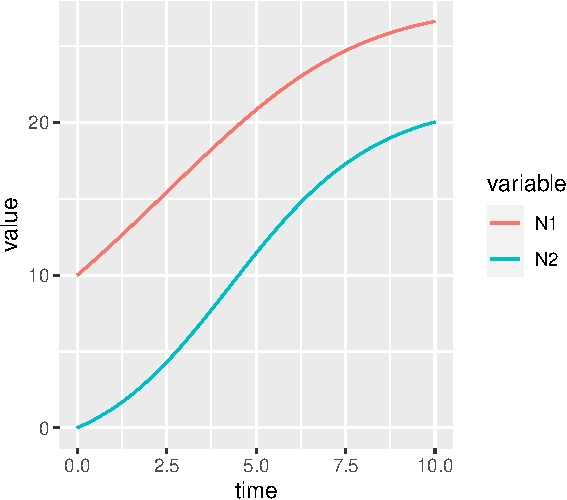
\includegraphics{deSolve_files/figure-beamer/unnamed-chunk-26-1.pdf}
\end{frame}

\hypertarget{una-representaciuxf3n-alternativa-de-la-trayectoria}{%
\subsection{Una representación alternativa de la
trayectoria}\label{una-representaciuxf3n-alternativa-de-la-trayectoria}}

\begin{frame}{Una representación alternativa de la trayectoria}
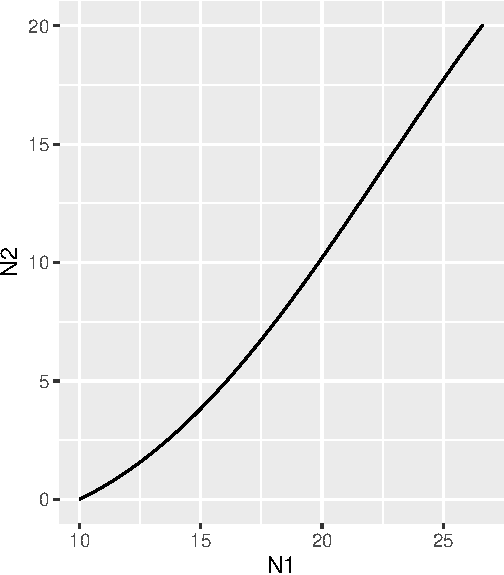
\includegraphics{deSolve_files/figure-beamer/unnamed-chunk-27-1.pdf}
\end{frame}

\end{document}
